\documentclass[final]{beamer}
\usetheme{RJH}
\usepackage[orientation=landscape,size=a1,scale=1.3,debug]{beamerposter}
\usepackage[absolute,overlay]{textpos}
\usepackage{amsmath}
\usepackage{mathtools}
\usepackage{commath}
\usepackage[font=scriptsize,labelfont=bf]{caption}
\usepackage{multicol}
\setlength{\TPHorizModule}{1cm}
\setlength{\TPVertModule}{1cm}
\setbeamertemplate{caption}[numbered]
\setbeamertemplate{itemize items}[ball]
\setbeamertemplate{bibliography item}{\insertbiblabel}
\usepackage{tikz}
\newcommand{\tikzcuboid}[4]{% width, height, depth, scale
\begin{tikzpicture}[scale=#4]
\foreach \x in {0,...,#1}
{   \draw (\x ,0  ,#3 ) -- (\x ,#2 ,#3 );
    \draw (\x ,#2 ,#3 ) -- (\x ,#2 ,0  );
}
\foreach \x in {0,...,#2}
{   \draw (#1 ,\x ,#3 ) -- (#1 ,\x ,0  );
    \draw (0  ,\x ,#3 ) -- (#1 ,\x ,#3 );
}
\foreach \x in {0,...,#3}
{   \draw (#1 ,0  ,\x ) -- (#1 ,#2 ,\x );
    \draw (0  ,#2 ,\x ) -- (#1 ,#2 ,\x );
}
\end{tikzpicture}
}

\newcommand{\tikzcube}[2]{% length, scale
\tikzcuboid{#1}{#1}{#1}{#2}
}


\title{\huge \vspace{0.2em}\\
Convolutional Neural Networks for 3D MNIST Image Classification\vspace{0.2em}}
\footer{}
\author{\huge Jeremy Irvin \\\vspace{0.4em}
\LARGE Stanford University\vspace{0.4em}
}
\date{}

\begin{document}
\begin{frame}{} 

\begin{textblock}{10}(2,3)

\includegraphics[width=4.5cm]{stanford.png}
\end{textblock}

\begin{textblock}{10}(76,3)

\includegraphics[width=6.5cm]{stanford2.png}
\end{textblock}

\begin{textblock}{24}(1,10)
\begin{block}{Motivation}
Visual object recognition is an essential skill for autonomous robots to function in real world environments. Robust classification of 3D digits is a crucial step towards this goal.
\end{block}


\begin{block}{Problem Definition}
Given a dataset of 10000 rotated and translated 3D point clouds with their digit labels from 0 to 9, automatically assign the correct digit to the 3D image without manual feature engineering.
\end{block}

\begin{block}{Background: Voxelization and Conv Nets}
\begin{figure}
\begin{center}
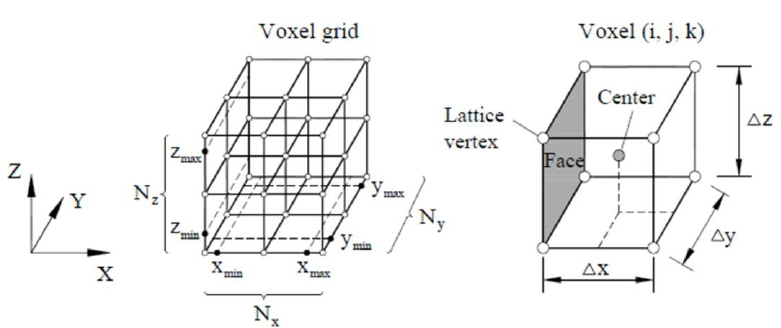
\includegraphics[width=23cm]{voxelgrid.png}
\end{center}
\vspace{0.5em}
\caption{Example of Occupancy Grid [1]. Each $(x,y,z)$ in the point cloud is assigned a single $(i,j,k)$ voxel. The image is then represented by a $N_x\times N_y\times N_z$ matrix where the $ijk$th entry contains the number of points assigned to that voxel.}
\label{voxel}
\end{figure}
\begin{figure}
\begin{center}
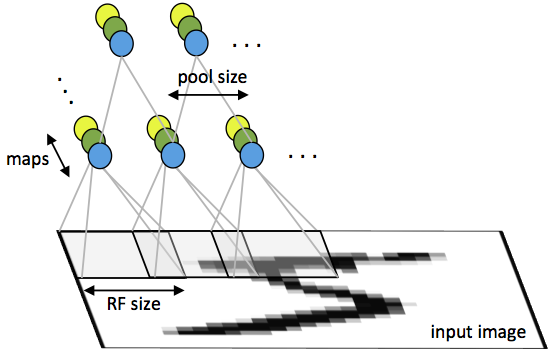
\includegraphics[width=14cm]{convolution.png}
\end{center}
\vspace{0.5em}
\caption{Example of the 2D convolution and pooling operations [2]. Units of the same color in the convolution layer share the same weights.}
\end{figure}
\vspace{-0.5em}
\end{block}
\end{textblock}

\begin{textblock}{30}(26.5,10)
\begin{block}{Data: 3D MNIST}
\begin{figure}
\begin{center}
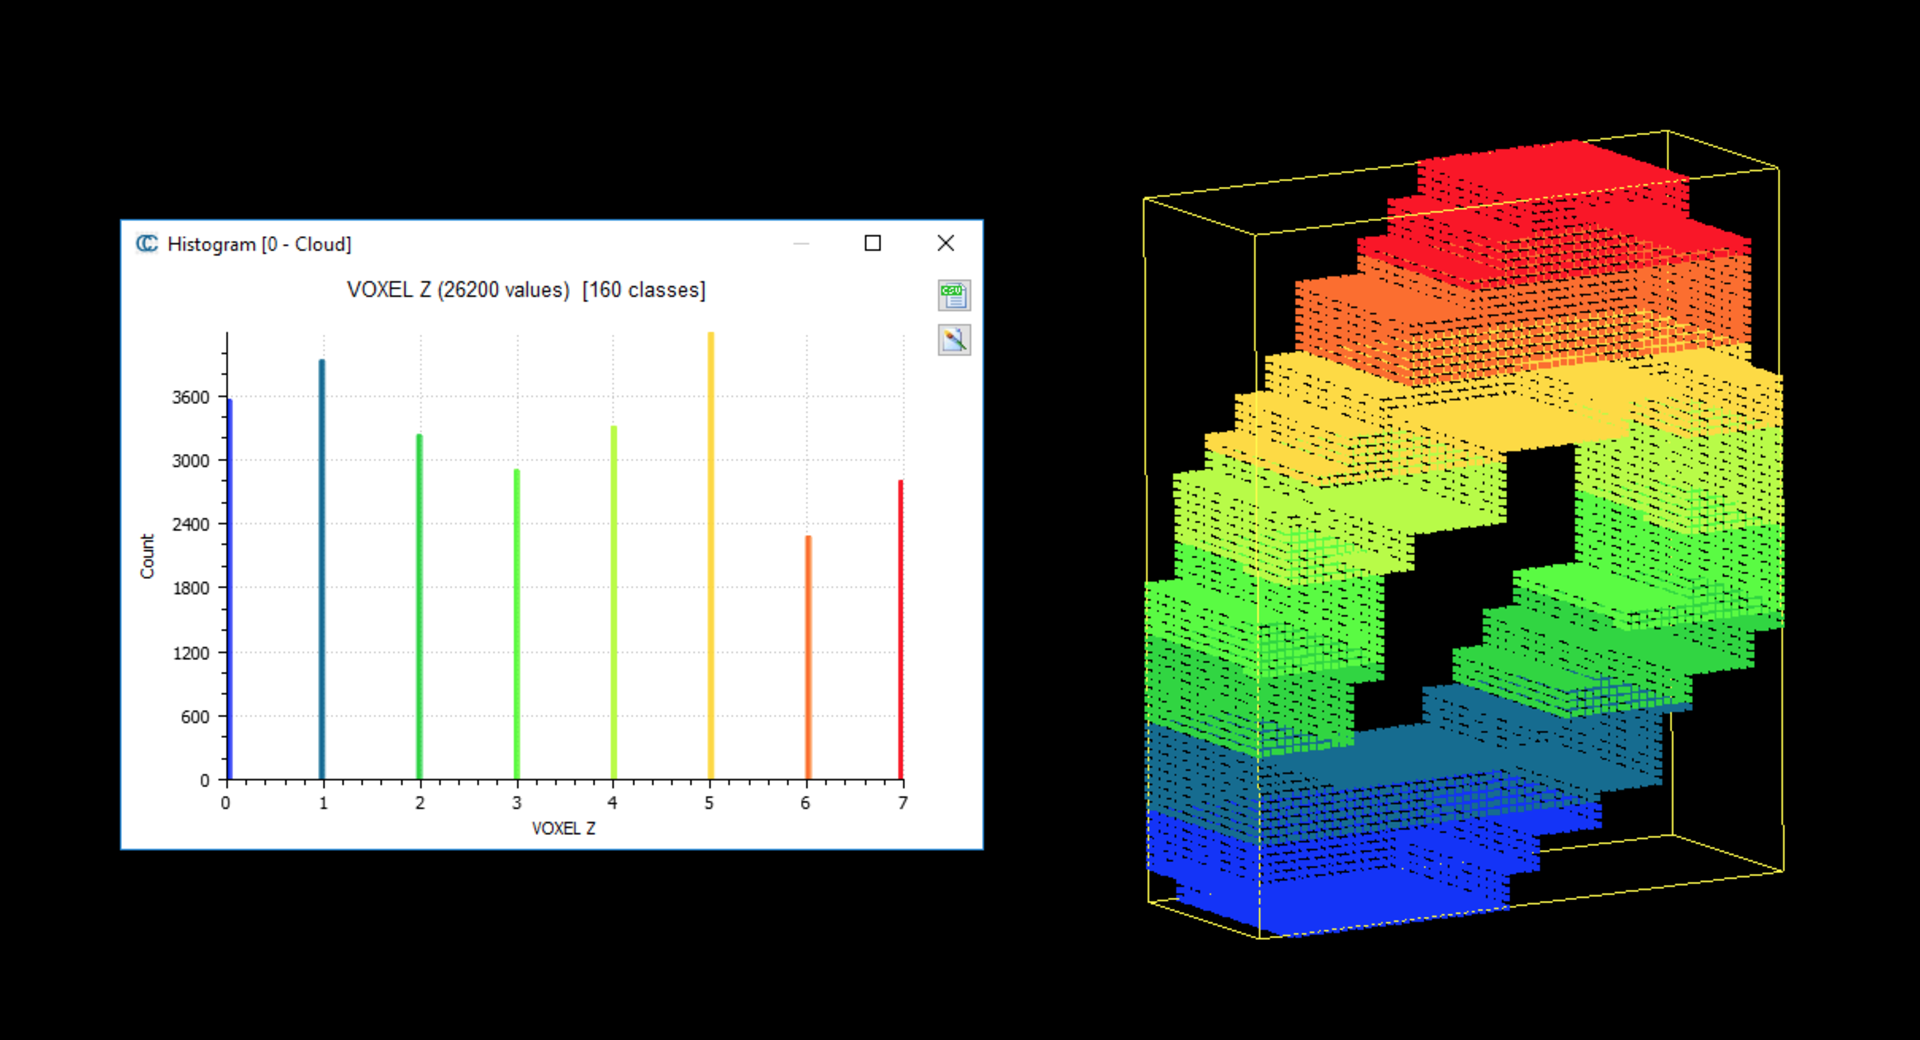
\includegraphics[width=14cm]{example_voxel.png}
\end{center}
\vspace{0.5em}
\caption{Example of an image split into 8 voxels along the $z$-axis (each color corresponds to a single voxel) [1]. The graph shows a count of points in each voxel in the $z$-dimension.}
\label{example}
\end{figure}
\begin{figure}
\begin{center}
\begin{tabular}{cc}
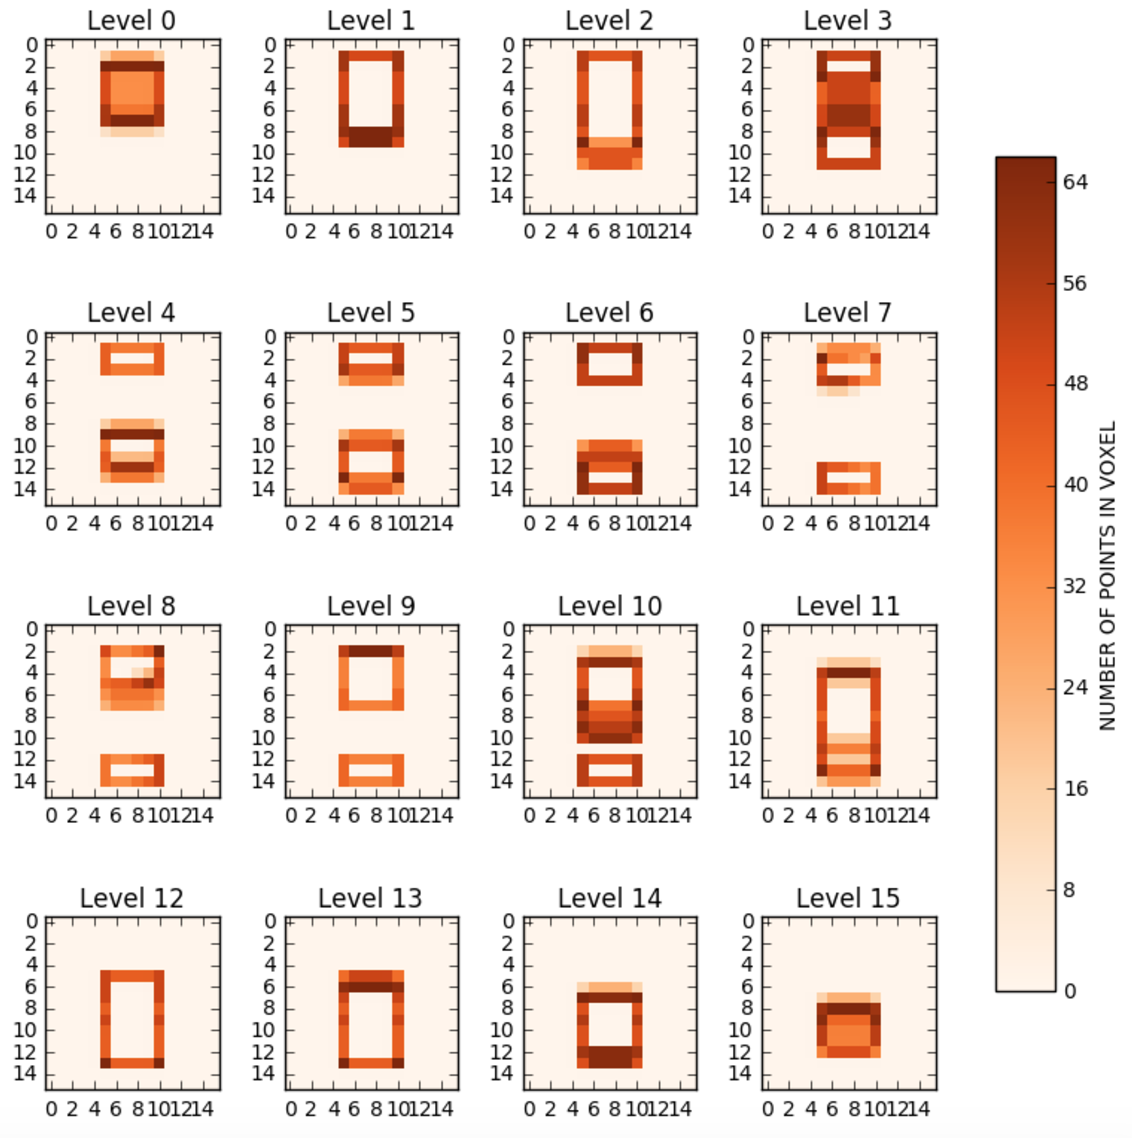
\includegraphics[width=7cm]{regular.png}&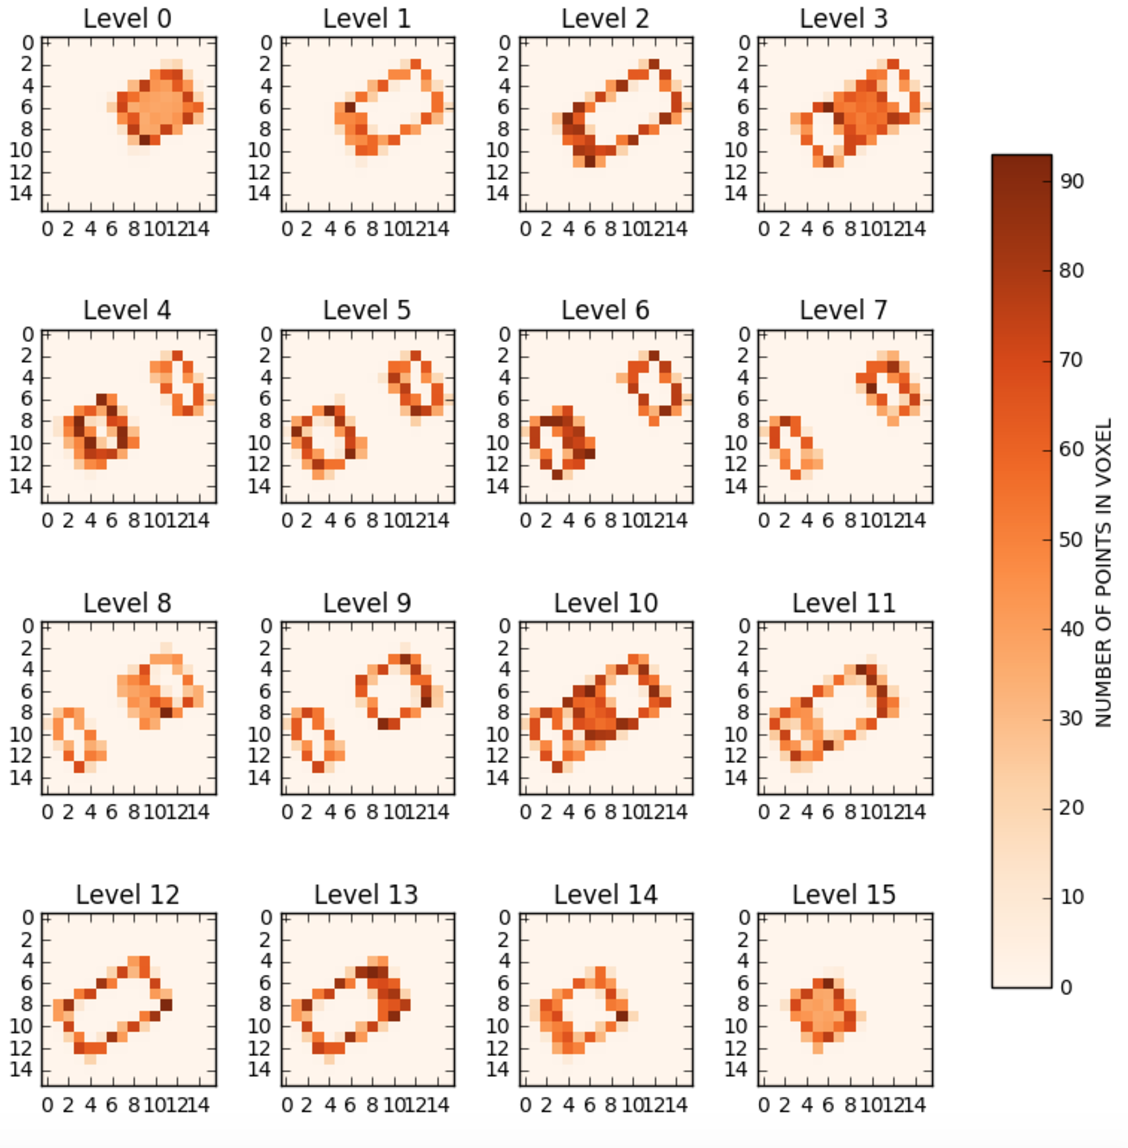
\includegraphics[width=7cm]{augment.png}
\end{tabular}
\end{center}
\caption{Example of rotation clockwise by $60^{\circ}$ along the $z$-axis [1]. The left panel shows a projection into the $x$ dimension (image axes are $z,y$ dimensions and levels are the $x$ dimension). The right panel shows the image rotated clockwise by $60^{\circ}$ in the $z$ dimension. The colors denote the number of points within a voxel.}
\label{augment}
\end{figure}
\vspace{-1em}
\end{block}

\begin{block}{Model: 3D Conv Net (VoxNet [3])}
\begin{figure}
\begin{center}
\begin{tikzpicture}
 \draw[blue] (9,3,2) -- (3,2,2);
 \draw[blue] (9,5,2) -- (3,4,2);
\foreach \x in{0,...,4}
{   \draw (0,\x ,4) -- (4,\x ,4);
    \draw (\x ,0,4) -- (\x ,4,4);
    \draw (4,\x ,4) -- (4,\x ,0);
    \draw (\x ,4,4) -- (\x ,4,0);
    \draw (4,0,\x ) -- (4,4,\x );
    \draw (0,4,\x ) -- (4,4,\x );
}
    \draw[line width=0.75mm] (1,4,4) -- (3,4,4);
    \draw[line width=0.75mm] (1,4,3) -- (3,4,3);
    \draw[line width=0.75mm] (1,4,2) -- (3,4,2);
    \draw[line width=0.75mm] (1,4,4) -- (3,4,4);
    \draw[line width=0.75mm] (3,4,2) -- (3,4,4);
    \draw[line width=0.75mm] (2,4,2) -- (2,4,4);
    \draw[line width=0.75mm] (1,4,2) -- (1,4,4);
    \draw[line width=0.75mm] (3,2,4) -- (3,4,4);
    \draw[line width=0.75mm] (2,2,4) -- (2,4,4);
    \draw[line width=0.75mm] (1,2,4) -- (1,4,4);
    \draw[line width=0.75mm] (1,2,4) -- (3,2,4);
    \draw[line width=0.75mm] (1,3,4) -- (3,3,4);
    \draw[line width=0.75mm, dotted] (3,2,2) -- (3,2,4);
    \draw[line width=0.75mm, dotted] (3,2,2) -- (3,4,2);
    \draw[line width=0.75mm, dotted] (3,2,3) -- (3,4,3);
    \draw[line width=0.75mm, dotted] (3,3,4) -- (3,3,2);
    
    \draw[line width=0.5mm,red] (7,5,4) -- (9,5,4);
    \draw[line width=0.5mm,red] (7,5,3) -- (9,5,3);
    \draw[line width=0.5mm,red] (7,5,2) -- (9,5,2);
    \draw[line width=0.5mm,red] (7,5,4) -- (9,5,4);
    \draw[line width=0.5mm,red] (9,5,2) -- (9,5,4);
    \draw[line width=0.5mm,red] (8,5,2) -- (8,5,4);
    \draw[line width=0.5mm,red] (7,5,2) -- (7,5,4);
    \draw[line width=0.5mm,red] (9,3,4) -- (9,5,4);
    \draw[line width=0.5mm,red] (8,3,4) -- (8,5,4);
    \draw[line width=0.5mm,red] (7,3,4) -- (7,5,4);
    \draw[line width=0.5mm,red] (7,3,4) -- (9,3,4);
    \draw[line width=0.5mm,red] (7,4,4) -- (9,4,4);
    \draw[line width=0.5mm,red] (9,3,2) -- (9,3,4);
    \draw[line width=0.5mm,red] (9,3,2) -- (9,5,2);
    \draw[line width=0.5mm,red] (9,3,3) -- (9,5,3);
    \draw[line width=0.5mm,red] (9,4,4) -- (9,4,2);
    
    \draw[blue] (9,5,4) -- (3,4,4);
    \draw[blue] (7,5,4) -- (1,4,4);
    \draw[blue] (7,5,2) -- (1,4,2);
    \draw[blue] (9,3,4) -- (3,2,4);
    \draw[blue] (7,3,4) -- (1,2,4);
\end{tikzpicture}
\end{center}
\vspace{0.5em}
\caption{3D Filter and Pooling operations on a simple $4\times 4\times 4$ image [4]. The $2\times 2\times 2$ cube on the right can be thought of as either the filter or the pool. This figure does not show the stride parameter - this is just the size of the shift of the filter or pool (a sliding window).}
\label{3d_conv}
\end{figure}
\vspace{-0.5em}
\begin{figure}
\begin{center}
\includegraphics[width=20cm]{network.png}
\end{center}
\caption{Basic network architecture. One convolutional layer, max pooling layer, fully connected layer, and last fully connected layer into the 10 classes, where a final softmax is performed. Cross entropy loss is used and trained in Tensorflow with an Adam optimizer.}
\label{network}
\end{figure}
\vspace{-1em}
\end{block}

\end{textblock}

\begin{textblock}{25}(58,10)
\begin{block}{Experiments and Results}
\begin{figure}
\begin{center}
\tiny
\begin{tabular}{|l|l|}
\hline
Model & Validation Accuracy\\
\hline
Linear multiclass ovr SVM: L2 Regularization, Squared Hinge Loss & 0.5635\\ 
\hline
Linear multiclass ovr SVM: L1 Regularization, Squared Hinge Loss & 0.5645\\  
\hline
Linear multiclass ovr SVM: L2 Regularization, Hinge Loss & \textbf{0.566}\\
\hline
RBF kernel multiclass ovr SVM & 0.5295\\
\hline
Polynomial kernel multiclass ovr SVM & 0.107\\
\hline
Sigmoid kernel multiclass ovr SVM & 0.496\\
\hline
ovr Logistic Regression: & \textbf{0.582}\\
\hline 
Multinomial Logistic Regression & 0.5805\\
\hline
2 Layer Neural Network, 512 Hidden Dimension & 0.667\\
\hline
2 Layer Neural Network, 1024 Hidden Dimension & \textbf{0.6785}\\
\hline
Oracle (Vanilla CNN) & 0.992\\
\hline
\end{tabular}
\end{center}
\vspace{0.5em}
\caption{Summary of baseline results. ovr stands for \textit{one-versus-rest} ($10$ binary classifiers). In the SVM case, ovr is contrasted with a \textit{one-versus-one} scheme ($\binom{10}{2}=45$ binary classifiers). In the Logistic Regression case, ovr is contrasted with Multinomial Logistic Regression, which is softmax regression with cross-entropy loss. The best SVM, logistic regression, and neural network classifiers are bolded. The oracle is a vanilla convolutional neural network which uses the 2D image that was used to generate the 3D point clouds.}
\label{baselines}
\end{figure}
\tiny
\begin{figure}
\begin{center}
\begin{tabular}{|l|l|}
\hline
Model & Validation Accuracy\\
\hline
3DConvNet: 1 layer, 8 filters, 1024 hidden dim & \textbf{0.69}\\
\hline
\end{tabular}
\end{center}
\caption{Summary of results.}
\label{results}
\end{figure}
\end{block}
\begin{block}{Future Work}
\begin{itemize}
\item\text{ }Further experiments using more complex architectures
\item\text{ }Visualize cross sections of filters and activation of fully connected layers
\end{itemize}
\end{block}

\begin{block}{References}
%{\tiny
%\bibliography{mybib}}
\footnotesize
[1] https://www.kaggle.com/daavoo/d/daavoo/3d-mnist/\\

[2] http://ufldl.stanford.edu/tutorial/supervised/ConvolutionalNeuralNetwork/\\

[3] http://www.dimatura.net/extra/voxnet\_maturana\_scherer\_iros15.pdf\\

[4] https://ai2-s2-pdfs.s3.amazonaws.com/3c86/dfdbdf37060d5adcff6c4d7d453ea5a8b08f.pdf
\end{block}
\end{textblock}

\end{frame}
\end{document}
